\chapter{Schematy działania systemu}
\label{cha:schematy}

Pierwszym etapem symulacji było przygotowanie środowiska symulacyjnego. Na zainicjalizowanej dyskretnej siatce \ref{figure:siatka}, zostali wygenerowani piesi oraz przeszkody. W symulacji wykorzystano śmioelementowe sąsiedztwo Moore'a \ref{figure:siatka}.

[Do dokończenia po zaimplementowaniu całości]
\begin{figure}
\label{figure:siatka}
\centering
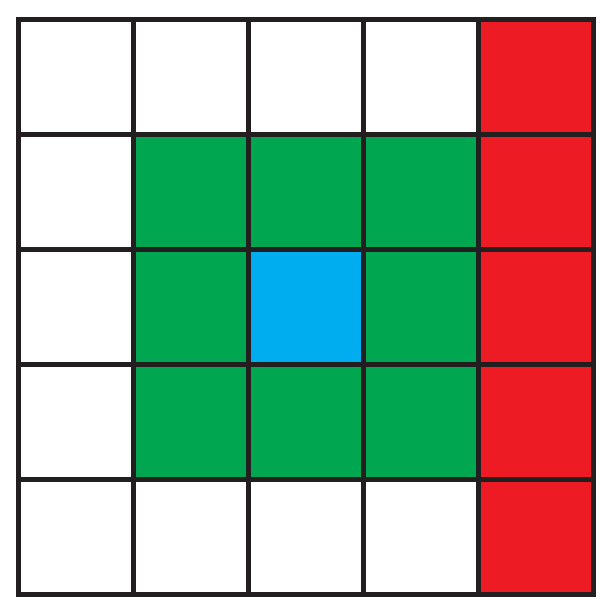
\includegraphics[width=0.4\textwidth]{sasiedztwo.eps}
\caption{Schemat siatki używanej w projekcie. Kolorem niebieskim oznaczono pieszego, zielonym jego sąsiedztwo Moore'a, czerwonym przykładowa przeszkoda}
\end{figure}

Symulacja została zaimplementowana przy użyciu języka Java w wersji 8 we wsparciu biblioteki graficznej Jwjgl.

\section{Przyjęte parametry}
[Do dokończenia po zaimplementowaniu całości]
